\chapter{Overview}
\label{chap:Overview}
\section{State of the art}
\label{sec:StateArt}
In this section we present the state of the art of the current knowledge of ventral striatum (VS) and ventral tegmental area (VTA), needed for the study of VS-VTA interaction.\\In VTA, dopamine neurons fire phasically (100-500 ms) after unpredicted rewards or cues that predict reward. Their response to reward is reduced when a reward is fully predicted (\cite{Uchida}). %Furthermore, their activity is suppressed when a predicted reward is omitted. From these observations, previous studies hypothesized that dopaminergic neurons signal discrepancies between expected and actual rewards (i.e., they compute RPE).
The uncertainty about the reward outcome is critical in the measure of information and in assessing the accuracy of predictions. The uncertainty is determined by the probability P to get the reward, and its maximal at $P=0.5$ decreases at higher and lower probabilities.\\Fiorillo and his collaborators used distinct stimuli indicating the probability of reward to show that the phasic activation of dopamine neurons varied monotonically across the full range of probabilities (\cite{Fiorillo}). These observations picked scientists$'$ curiosity, who showed growing interest on dopamine signals. Further studies showed that dopamine neurons signal discrepancies between expected and actual rewards, in other words they compute the reward prediction error (RPE).\\Figure \ref{fig:Fiorillo} displays the dopamine neurons response to stimuli with different reward probability.%In stark contrast to the simple models proposed previously, we observed that information about reward and expectation is distributed among multiple brain areas and already mixed in many individual input neurons. Our data suggest that the RPE computation is not a one-step process combining pure information about reward and expectation in dopamine neurons. Nor do dopamine neurons receive complete RPE from a specific brain area. Instead, the coexistence of input neurons encoding pure and mixed information, some of which are partial and complete RPE signals, appears to be a sign of redundant computations distributed in a complex neuronal network that ultimately converge onto dopamine neurons to construct a more complete RPE signal.
\begin{figure}
    \centering
    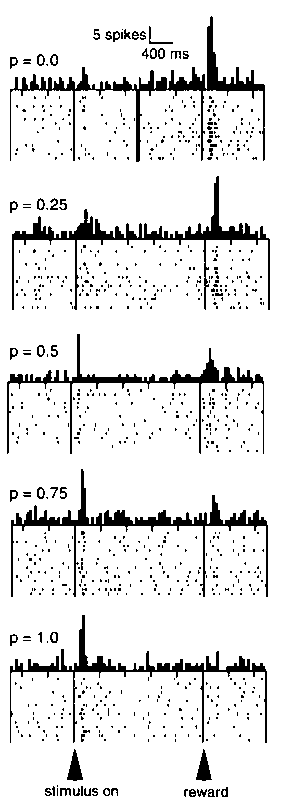
\includegraphics[scale=0.8]{figures/Schultz1.png}
    \caption{Adapted from \cite{Fiorillo}. Reward-related response of dopamine neurons. Distinct stimuli were used to indicate the probability of reward (P increasing from top to bottom). Dopamine neurons signals varied monotonically across the full range of probability. At the stimulus onset the dopamine response increased monotonically as the probability increased, at the reward time instead the dopamine response decreased monotonically as the probability increased}
    \label{fig:Fiorillo}
\end{figure}
\begin{figure}
    \centering
    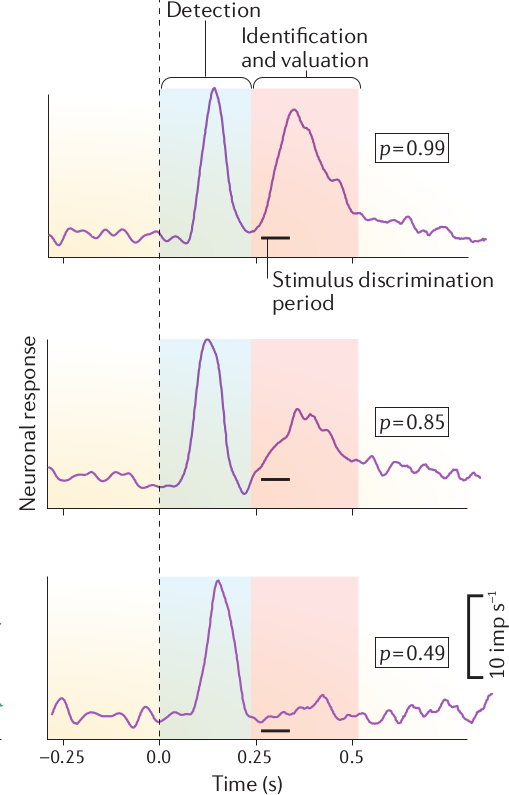
\includegraphics[scale=0.4]{figures/ResponseProbSchultz.png}
   % 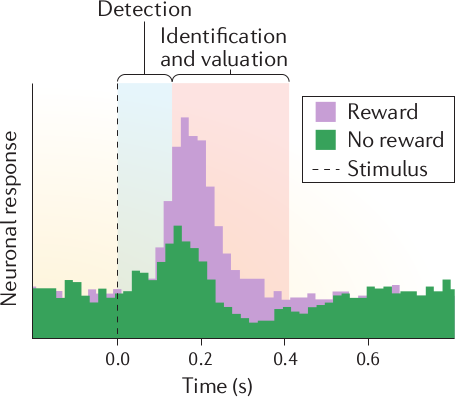
\includegraphics[scale=0.4]{figures/Schultz2016CSMod.png}
    \caption{Adapted from \cite{Schultz2016}. A demanding random dot motion discrimination task reveals completely separated dopamine response components. Higher response corresponds to higher reward probability (p). The initial, stereotyped, non-differential activation reflects stimulus detection and decreases back to baseline (blue zone); the subsequent separate, graded increase develops when the animal signals stimulus discrimination; it codes reward value (red zone), which in this case derives from reward probability}
    \label{fig:probSchultz}
\end{figure}
More in detail, several studies have shown that RPE signal evolves in time from unselective sensory detection to more demanding and crucial stages of identification and valuation (\cite{Tobler2003}, \cite{Nomoto2010}, \cite{Fiorillo2013}, \cite{Schultz2016}), value that is constantly adapted during the learning process by dopamine neurons (\cite{Tobler2005}). The initial component, characterized by a brief activation, occurs unselectively in response to a large variety of unpredicted events and corresponds to the large range and heterogeneous nature of potentially rewarding stimuli and object present in the environment. This component reflects the detection of stimulus, regardless its relation with the reward.\\The second component, also called main component or valuation component, defines the function of the dopamine response and reflects the evolving neuronal processing that is required to fully appreciate the value of the stimulus. Thus, at this stage the stimulus is identified and valued. Figure \ref{fig:probSchultz} shows the separation between the detection salience and the valuation component of RPE in dopamine  signals.\\Like VTA neurons, VS neurons show as well reward-related response. In monkey experiments first it has shown that VS neurons predominantly fire in relation to the expectation of reward, regardless the movement no-movement reaction (\cite{Schultz1992}). This signals suggested that VS neurons have access to central representations of reward and thereby participate in the processing of information underlying the RPE computation.\\The stereotypical response of projection neurons in VS during learning consists in a sustained increase of activity before the occurrence of the reward delivery (see figure \ref{fig:StriatumN}).
\begin{figure}[H]
    \centering
    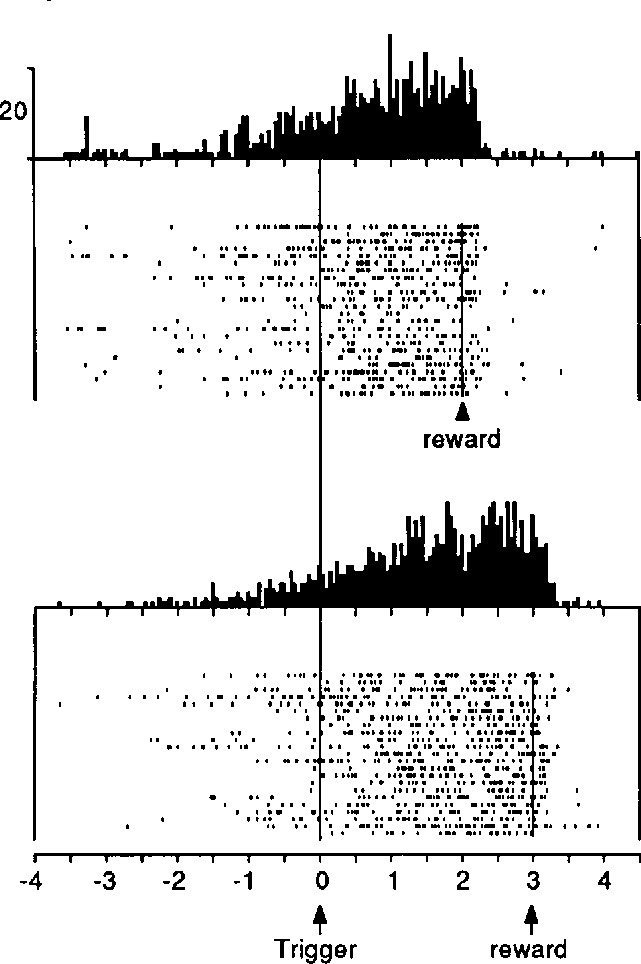
\includegraphics[scale=0.3]{figures/StriatumR.png}
    \caption{Adapted from \cite{Schultz1992}. Stereotypical reward-related VS neuronal activity. Effect of delayed reward delivery in no/ no go task in monkeys. VS neurons showed sustained increases of activity before the occurrence of individual task events. VS neurons exhibit activation in relation to the expectation of reward.}
    \label{fig:StriatumN}
\end{figure}
The ventral pallidum (VP), from which we recorded fast spiking activity, is innervated by dopamine inputs from the midbrain and dopamine directly alters VP neuronal firing (\cite{Napier89}). Since 1991 VP was assumed to integrate reward-related signals carried by VTA dopamine neurons, involved in reward-motivated behavior (\cite{Napier91}). This concept was quickly expanded to encompass the idea that dopamine transmission within the VP regulates a collection of behaviors, including locomotion and cognition (\cite{Napier92}). For these reason, the responses of VP neurons are expected to be diverse among different VP units, depending on their involvement in a specific coding.
\section{Experiment and data set}
\label{sec:Dataset}
In this session we describe the experiment and the collected data for the analysis in object in this work. The experiment and the single units classification was conducted by Max Scheller, medical student, member of the Kelsch group.\\
The task presented is a go/no-go reversal odor discrimination task (see details in \hyperref[sec:MatAndMet]{~Section\ref*{sec:MatAndMet}}). In figure\ref{fig:experiment} the scheme of the experimental set-up. Dual-site in-vivo data were recorded in ventral striatum and ventral tegmental area, while two odors were presented to head-fixed mice, one rewarded (CS+) with reward probability 0.9, the second one unrewarded (CS-). Learning the task consisted in licking at least a defined number of times (two or three depending on the paradigm) during a specific interval, called lick window, when the rewarded odor (CS+) was presented (hit trials) and not licking when unrewarded odor (CS-) was presented (correct rejection trials). Whereas a bad performance consisted in not licking, or licking outside the lick window period, at CS+ presentation (miss trials), or licking at CS- presentation (false alarm trials). Once the performance criterion was reached, the contingencies were switched, in other words the rewarded odor became unrewarded and vice-versa. Once the performance criterion was reached in the reversal phase the extinction phase followed, in which neither one of the two odors was rewarded. The lick window was open for an interval ranging from 1500 $ms$ to 2000 $ms$ depending of different paradigms. after a delay from 500 $ms$ to 1500 $ms$. Only licks happening in the lick window interval were counted as valid to get the reward.\\
\begin{figure}[H]
    \centering
    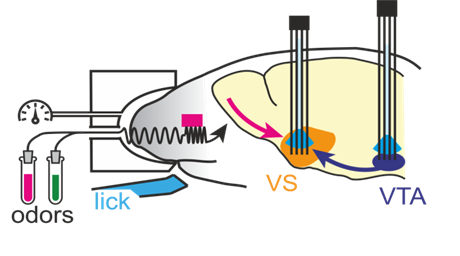
\includegraphics[scale=1.2]{figures/Experiment.png}
    \caption{Scheme of the experimental setup. Two odors in randomized sequences were presented, the mouse was head-fixed and, to get the reward, had to lick during the allowed licking period when the rewarded odor was presented. Electrodes were implanted in ventral striatum and ventral tegmental area to record the neural activity.}
    \label{fig:experiment}
\end{figure}

\begin{figure}[H]
    \centering
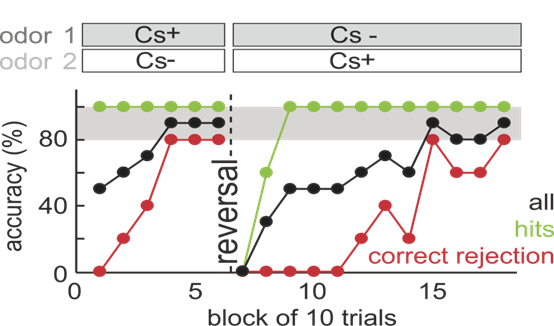
\includegraphics[scale=1]{figures/Performance.png}
\caption{Example of one animal's performance in original and reversal phase. In the shown paradigm the performance criterion to be reached to switch to the reversal phase was $79\%$, meaning that this level of accuracy had to be satisfied for hit trials and correct rejection trials. Black line indicates global performance including hit trials and correct rejection trials. Green line is the performance for the performance in hit trials and red lines is the performance in correct rejection trials.}
\label{fig:performance}
\end{figure}
\section{Materials and Methods}
\label{sec:MatAndMet}
\subsection{Data acquisition}Neural data was recorded with a 64-channel headstage (RHD2164) and interface board (RHD2000) by Intan Technologies LLC at 30 kHz sampling frequency. The same interface was used to record stimulus onset and offset, reward application, licking activity and laser stimulation.
\subsection{Probe Design}
Given the relatively high distance ($>6 mm$) between sites, depth of the target structures ($>5 mm$) and curvature of the OT/VP,  we developed a probe design specifically attuned to these challenges and easily adaptable to different single- or multi-site configurations. A detailed tutorial for the streamlined successor version of the implant used here is in preparation. The design exploits the high precision of the mature production technology of printed circuit boards (PCB)  ($\pm10\mu m$, custom-designed boards ordered from Wuerth Electronics) to achieve a precise x-y-placement of the guiding channels for optical fibers (Thorlabs \#) and tetrodes (spun from $12.5 \mu m$ teflon-coated tungsten wire, California Fine Wire). For the VTA, four tetrodes were attached to an optical fiber and fixed in their guiding channel.  For the OT/VP, the implant was placed above a mould of the ventral brain surface, and tetrodes and an optical fiber were advanced to their z-position and fixed in place, matching the bowl-shaped 3d-curvature of the OT (see pictures). Single tetrode wires were attached to the PCB using gold pins (Neuralynx). The connection between PCB and head stage was made via a Molex SlimStack connector (mated height: 1 mm, pitch: 0.4 mm, 70 channels, \# $502426-7030$) and an custom adaptor to the 2x36 Omnetics Nano Strip connectors of the Intan RHD2164 head stage.\\ 
\begin{figure}
    \centering
    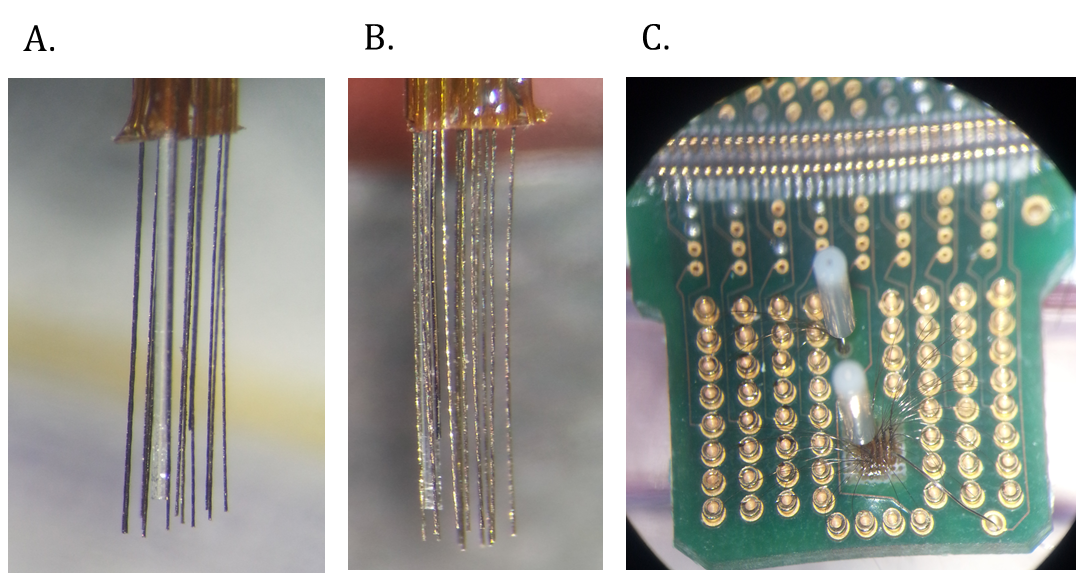
\includegraphics[scale=0.4]{figures/Implant.png}
    \caption{Foto provided by Max Scheller.}
    \label{fig:implant}
\end{figure}
\subsection{Animals and surgery details}
18 adults mice(DAT:Cre$+$, ChR2:YFP$+$ )(5-6 months aged) were implanted. The surgery duration was less than 2 hours, after which mice were housed individually. The recovery period was one week.\\
After termination of the experiments, animals were deeply anaesthetized with isofluorane and transcardially perfused with%[x$\%$]
formaldehyde solution. Placement of tetrodes in the target areas was evaluated post mortem by first explanting the whole brain, dorsal skull and attached probe as a unit, documenting the ventral aspect, where tetrode tips could be seen through the surface of the OT (foto\ref{fig:surgery}, left), and, in some cases, breaching it (foto\ref{fig:surgery}, right). After that, the relevant hemisphere was sectioned ($100 \mu m$) sagitally with a microtome (model \#) and mounted serially, so tetrode tracks could be traced.
\begin{figure}[h!]
    \centering
    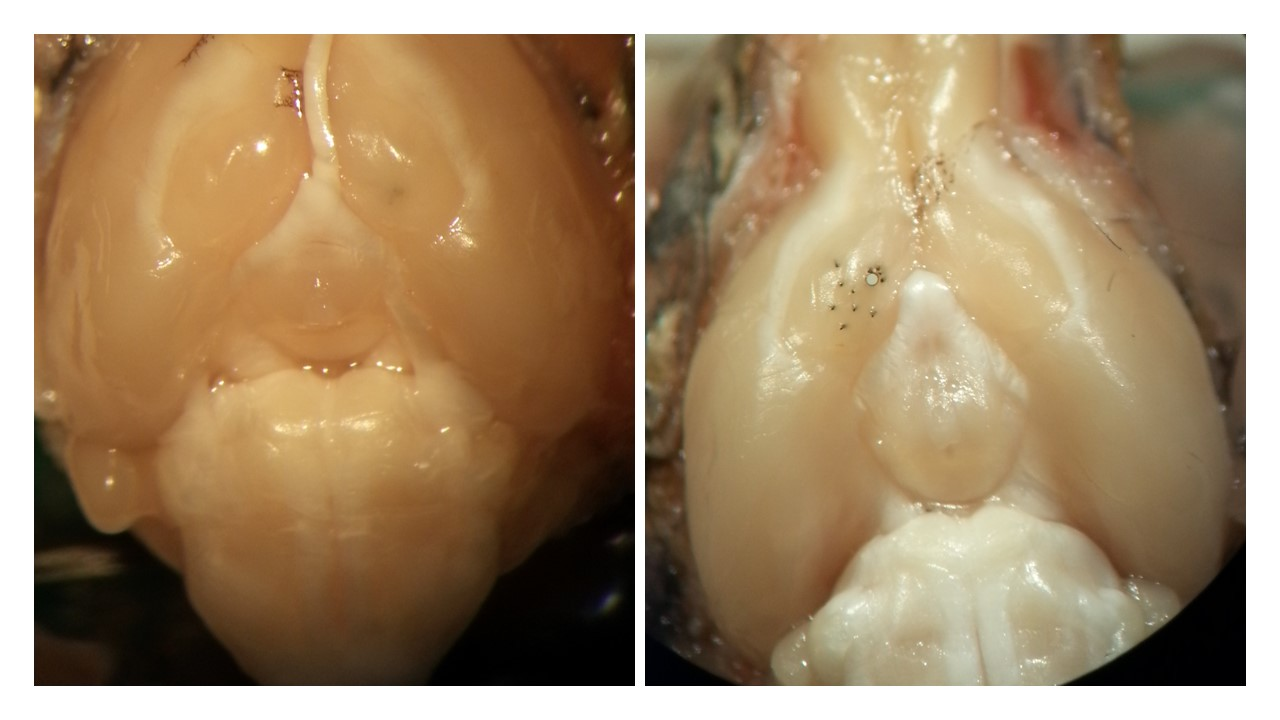
\includegraphics[scale=0.2]{figures/surgery_3.jpg}
    %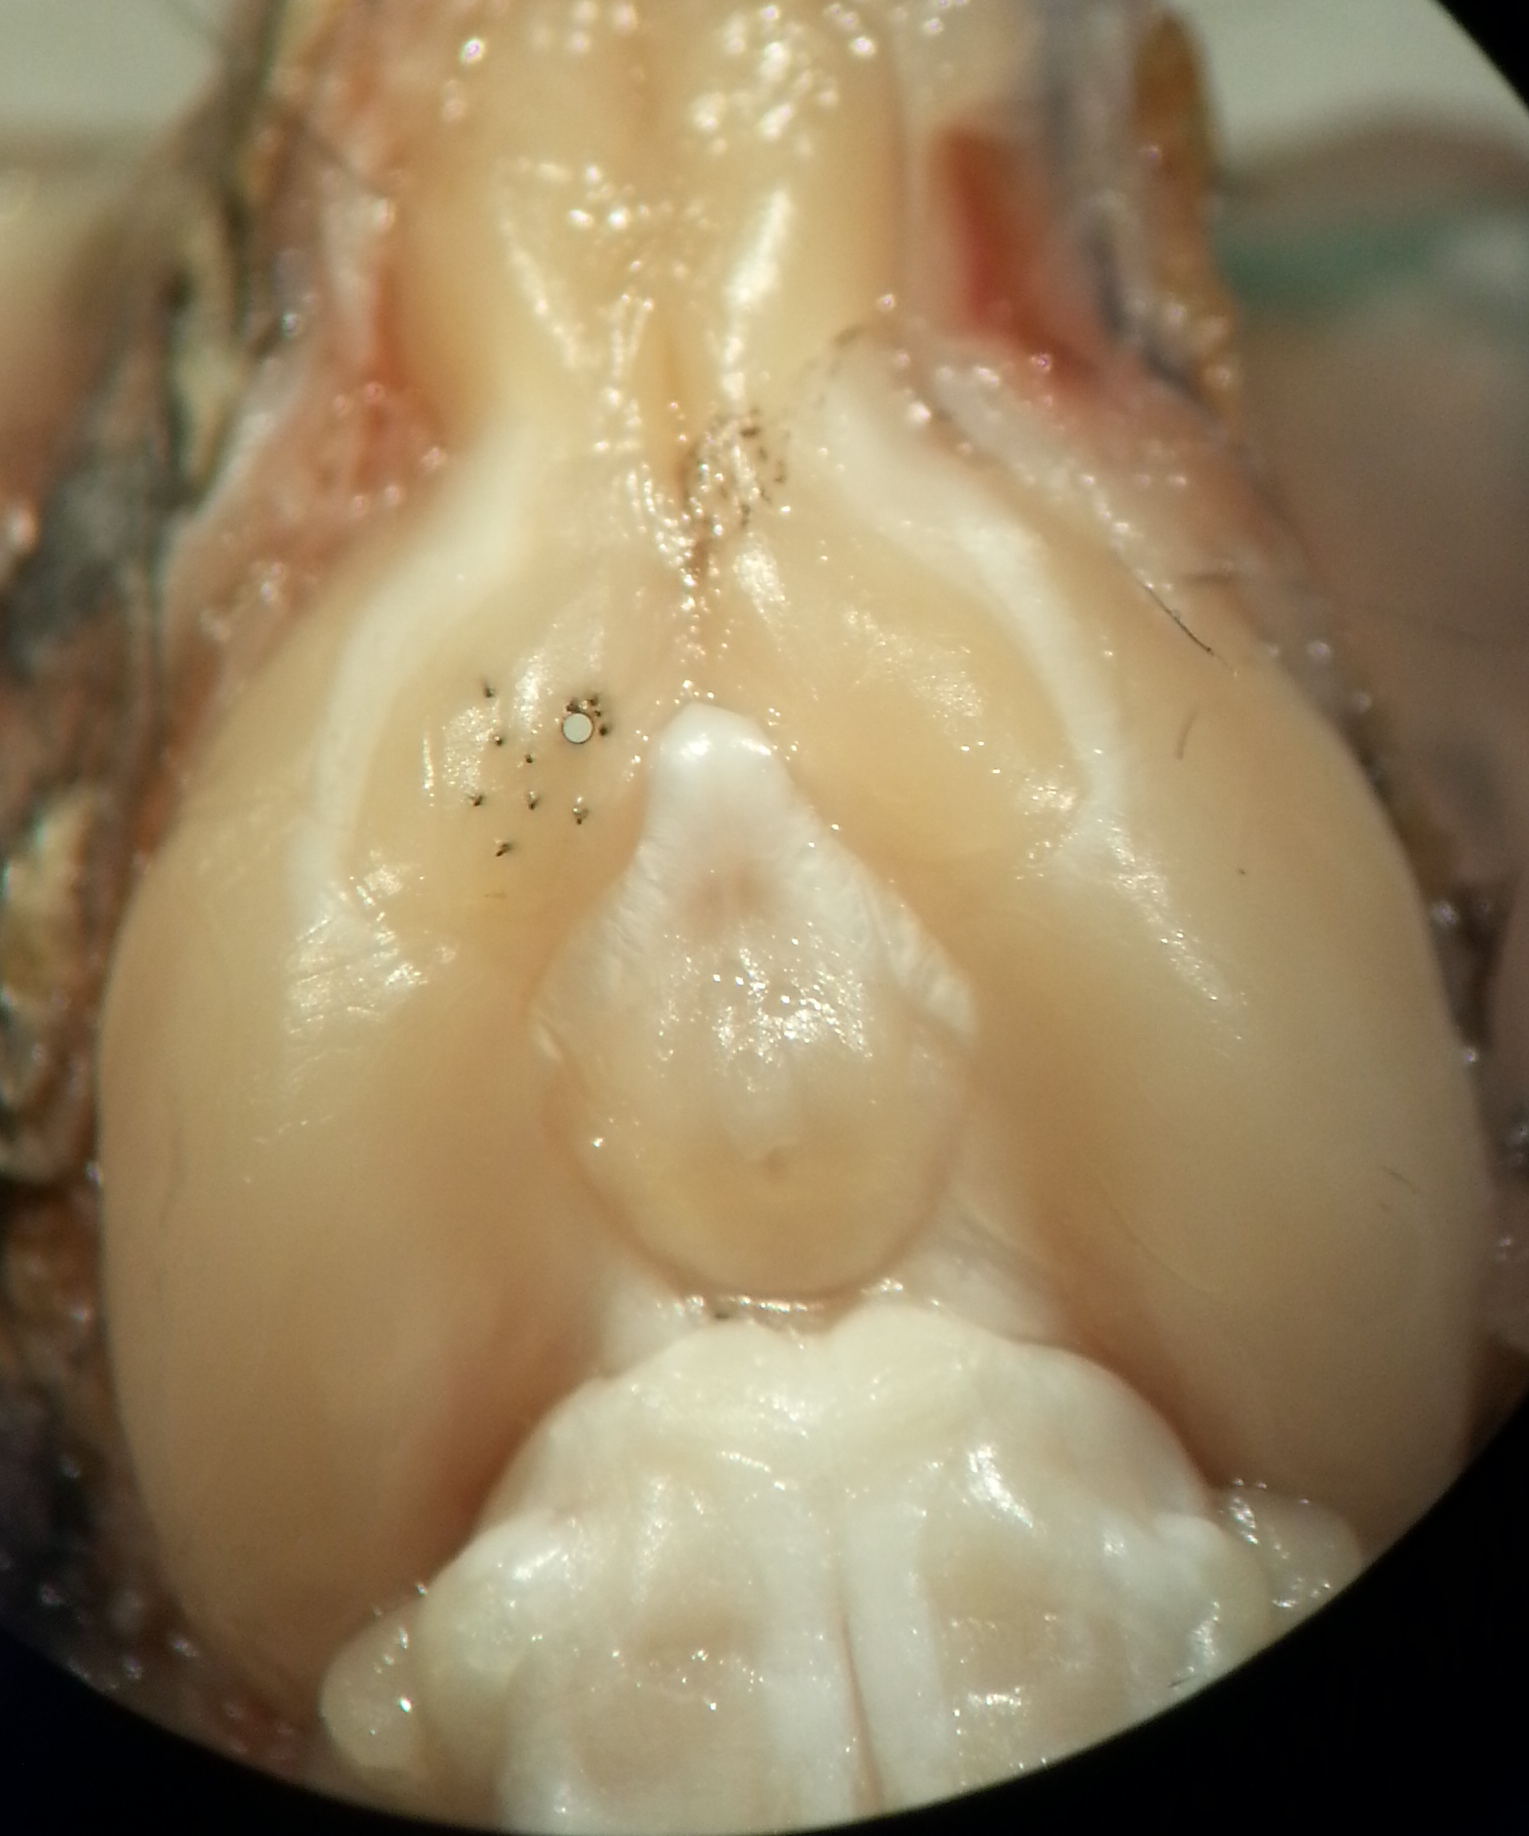
\includegraphics[scale=0.1]{figures/Surgery2.png}
    \caption{Foto provided by Max Scheller}
    \label{fig:surgery}
\end{figure}
\subsection{Behavioral conditioning in the go/no-go task.} We trained the animals in the head-fix setup described above. Mice received water in their home cage so that their body weight stabilized at 85$\%$ of baseline body weight. The training comprised multiple stages and progressed after reaching a performance criterion defined as at least 80$\%$ correct responses in 50 consecutive trials. Trials were considered correct if either at a $'$go$'$-response the reward was retrieved or at a $'$no-go$'$-response no significant licking was detected during the lick window. In the initial sessions, the animals’ licking behavior was shaped by first presenting them with a drop of water and subsequently letting them obtain more water when they licked at the licking spout (available in a random interval schedule, 0.5-12 s). Stage 1 ($'$training$'$): A single odorant (1.5 s stimulus duration) was presented. Animals could obtain a 5 $\mu l$ drop of water if they licked at least three times during a window from 0 to 2.5 s after stimulus onset (‘retrieval window’), this was considered a $'$go$'$-response. The interval between trials was randomly set at $10\pm 2$ s in all stages. Stage 2 ($'$discrimination$'$) consisted of two odorants in pseudo-random succession (no more than 3 consecutive trials with the same stimulus). One odorant (1.5s duration) was rewarded as in stage 1 (retrieval window: 0.5 – 2.5 s), while a $'$go$'$-response for the second odorant was registered as a false alarm and thus incorrect. No punishment was used. Stage 3 ($'$reversal learning$'$) used the same parameters as stage 2, but upon reaching the performance criterion (in the $'$original phase$'$), the reward contingency of the odors was switched ($'$reversal phase$'$). The data set used in this study consists of one reversal learning session per animal (10 sessions with a total yield of 75 single units) after we accustomed them gradually to a longer lick delay (1.5 – 3 s), keeping odorant delivery concurrent (3 s duration). 

\subsection{Data pre-processing: Spike detection.} To reduce noise and movement artifacts affecting all recording sites, we subtracted the median voltage trace of all channels from each recorded trace. The resulting signal was band pass filtered between 300 and 5000 Hz (4th order Butterworth filter, built-in MATLAB function). A threshold value for spikes was computed as a multiple (7.5x) of the median absolute deviation of the filtered signal (\cite{Quiroga}). Temporally proximal detected peaks over threshold were pruned by height to a minimum distance of 1 ms to avoid multiple detections of the same multiphasic spike. When an event was detected on multiple channels of a tetrode, the timestamp of the highest detected peak was used. Spike waveforms were extracted around $-10$ to $+21$ samples around the peak.

\subsection{Data pre-processing: Spike sorting.} Spike sorting was done with a custom-built graphical user interface in MATLAB, originally developed by A. Koulakov (CSHL). Metrics used for clustering included detected peak height or amplitude (and the respective principal components over channels), and the first three principal components of the waveforms for each respective channel when a spike was predominantly recorded on one channel. The quality of single unit clusters was assessed using the mlib toolbox by Maik Stuettgen (Vs. 6, $\href{https://de.mathworks.com/matlabcentral/fileexchange/37339-mlib-toolbox-for-analyzing-spike-data}{MLIB-toolbox-for-analyzing-spike-data}$) with particular attention to peak height distribution (fraction of lost spikes due to detection threshold), contamination (fraction of spikes during the refractory period $<5ms$) and waveform variance.\\
%For analysis of the silicon probe data, spike detection and spike sorting was done using KiloSort (\cite{Pachitariu}), followed by manual curation with Phy (\href{https://github.com/kwikteam/phy}{KiloSort}) using similar parameters to assess unit quality.\\
\subsection{Data pre-processing: Inclusion criteria of units.} For further analyses, units were only included if they complied with a set of criteria: Throughout the analyzed part of the recording session units were allowed to only have a maximum change in baseline firing rate from beginning to the end of the session of less than ten percent and intermittent maximum fluctuations of 20$\%$.\\ After exclusion of the first ten trials of odorant application where we frequently observed an initial response habituation, both odor responses had to be stable throughout the $'$pre$'$ phase.
\subsection{Optogenic tagging}
Identification of optogenetically modulated units was achieved by crosscorrelation of spike train and laser pulses.\\
After sessions, trains of 5 ms laser pulses (8-12 Hz, 5 mW) were delivered in either brain region via the implanted optical fibers. For each unit/region-pair, a test crosscorrelogram was computed from the timestamps of spikes and laser pulses (bin width: 1 ms, lag:  0-20 ms). To test for significant modulation, control crosscorrelograms ($n = 10000$) were constructed by shifting each laserpulse randomly in the interval $\pm$30ms around its original time, thus destroying any temporal relation on that timescale while preserving the properties of the spike train. Modulation was considered significant if two consecutive bins of the test crosscorrelogram lay outside of the middle 95$\%$ of the global distribution in the control crosscorrelograms. 
